\chapter{Модель персонального пространства в приложении SmartScribo}

%Парадигма ИП позволяет реализовывать приложения в совершенно различных предметных областях и одной из таких областей могут являтся блоги.
В данной главе рассматривается проект блог-клиента для мобильного устройства, использующего
парадигму ИП, описывается его архитектура, структура персонального пространства
блоггера и онтология для представления предметной области блогов.

\section{Приложение SmartScribo}

В настоящее время блоги являются одним из популярных видов социальных сетей. Блог --- это сетевой дневник, основным содержимым которого являются регулярно добавляемые записи, изображения или мультимедиа. Блог-сервисом называется сервер, предоставляющий работу с блогами для пользователей. Совокупность всех блогов в сети называется блогосферой. Для блогов характерны недлинные записи временной значимости, отсортированные в обратном хронологическом порядке (последняя запись сверху). Отличия блога от традиционного дневника обусловливаются средой: блоги обычно публичны и предполагают сторонних читателей, которые могут вступить в публичную полемику с автором (в комментариях к блог-записи или своих блогах).

Популярность блогов настолько высока, что миллионы пользователей публикуют свежую информацию о себе или обмениваются мнениями по различным темам. Данный феномен быстро становится частью жизни человека, и блогосфера является подходящей областью для экспериментов с использованием идей повсеместных вычислений \cite{karger:what,benson:talking}.

Существует множество клиентов, позволяющих работать с блогами, которые могут быть как браузерными, так и автономными. Автономные клиенты чаще всего используются на мобильных
устройствах, так как они обеспечивают более эффективную работу с блогами, чем мобильный браузер.
В таких клиентах обычно учитываются небольшие размеры экрана и клавиш устройства, а также ограниченность скорости сетевого трафика.

Проект SmartScribo \cite{smartscribo-old, smartscribo} представляет собой приложение, предназначенное для работы с различными блог-сервисами. Общая идея блоггинга в ИП представлена на рис. \ref{concept}. Множество блогов, хранящихся на блог-сервисах и представленных пользователю в HTML, отображаются в отдельные пространства в общем ИП и представляются в RDF-формате. Ключевой особенностью приложения является возможность мультиблоггинга,
которая позволяет пользователю работать одновременно с несколькими блогами.

\begin{figure}[h]
\centerline{
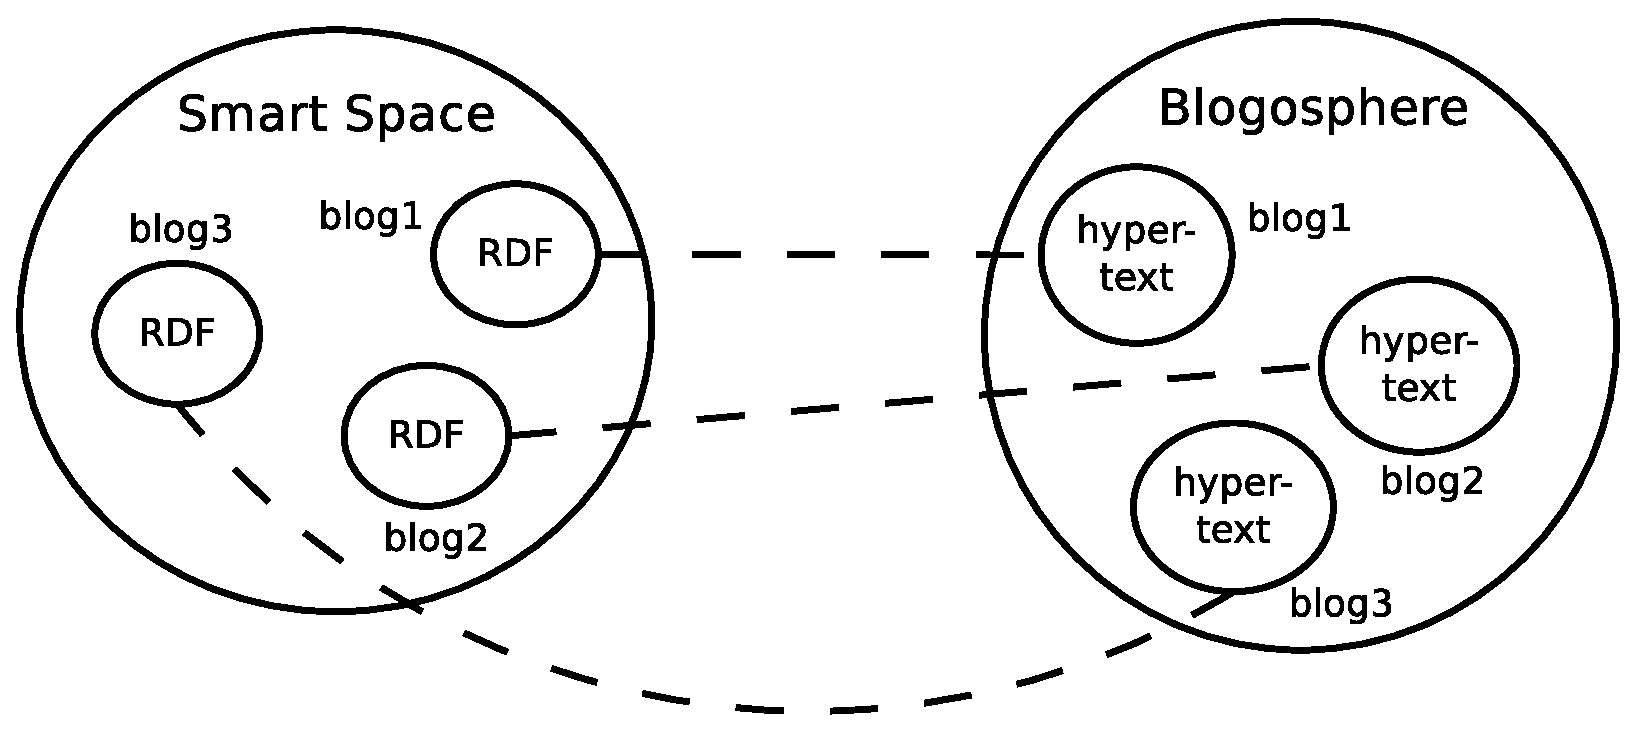
\epsfig{file=images/concept.eps, width=15cm}}
\caption{Схема блоггинга в ИП}
\label{concept}
\end{figure}

Основными возможностями приложения SmartScribo являются:
\begin{enumerate}
\item
Просмотр нескольких блогов пользователя, как единого блога.
\item
Получение, отправка, редактирование постов блога.
\item
Кросс-постинг: отправка поста в несколько блогов одновременно.
\item
Получение, отправка, редактирование комментариев поста.
\item
Сортировка и фильтрация списка постов.
\item
Просмотр блогов друзей.
\end{enumerate}

Однако клиент-серверная архитектура является недостаточно эффективной для релизации мультиблогового
клиента, особенно для мобильного устройства. Параллельная работа с несколькими блог-сервисами
приводит к быстрой разрядке аккумулятора и резкому снижению скорости сетевого траффика. 
Следовательно возникает необходимость использовать
альтернативную архитектуру, в качестве которой подходит архитектура приложений, основанных на парадигме ИП.

Распределённая архитектура SmartScribo (рис. \ref{scribo-architecture}),
основанная на концепции ИП, позволяет пользователю взаимодействовать с несколькими
блог-сервисами, а также предоставляет возможность работы нескольких клиентов одновременно. В приложении SmartScribo можно выделить три вида агентов.

\begin{figure}[h]
\centerline{
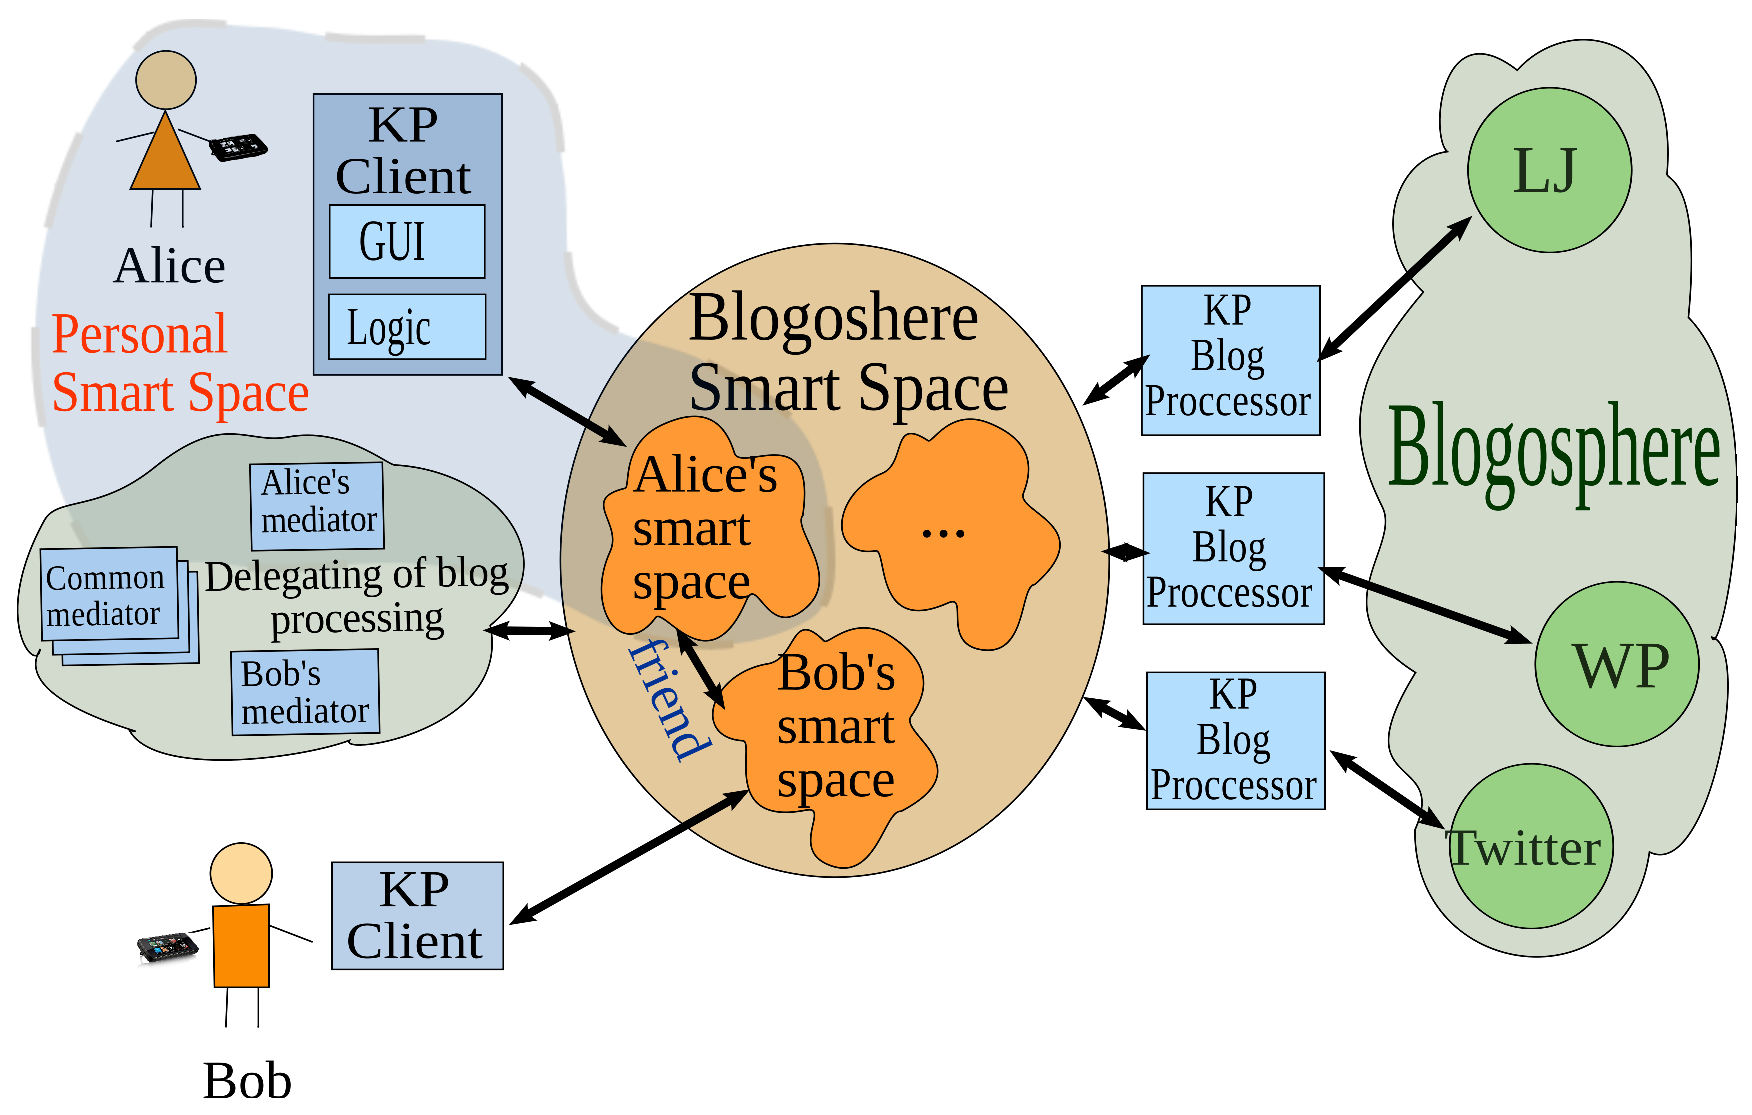
\epsfig{file=images/scribo_ss-arch.eps, width=15cm}}
\caption{Архитектура SmartScribo}
\label{scribo-architecture}
\end{figure}

{\bf 1. Клиентский агент (KP Client)} --- агент, запускающийся на пользовательском
устройстве. Клиентский агент позволяет пользователю работать с блогами и осуществляет данное взаимодействие через ИП.
Таких агентов может быть любое количество, и они могут быть запущены на различных устройствах: персональном компьютере, нетбуке или мобильном телефоне.

{\bf 2. Агент блог-процессор (KP Blog Processor)} --- агент, который взаимодействует с определённым блог-сервисом и обрабатывает запросы от всех клиентов. 
Блог-процессор работает с аккаунтами пользователей, посылает/получает посты и комментарии и частично отражает содержимое блогосферы в ИП.

{\bf 3. Агент медиатор (KP mediator)} --- данный агент предназначен для разного рода
обработки информации, хранящейся в ИП.
Агенты медиаторы могут быть как общими, т.е. использовать данные нескольких блоггеров, так и личными для каждого пользователя. В качестве примера функциональности медиатора могут служить такие операции, как оптимизация и удаление дублирующей информации в ИП или система рекомендаций, выполняющая поиск постов и предлагающая их прочитать пользователю на основе его интересов.

У каждого пользователя SmartScribo в глобальном ИП выделяется персональное пространство блоггера. Клиентский агент взаимодействует чаще всего именно с этим пространством, получая из него данные блогосферы.
Кроме этого агент блог-процессор при ответе на запрос клиента также размещает блог данные в пользовательское пространство. Таким образом взаимодействие между клиентскими агентами и блог-процессорами осуществляется именно через персональное пространство блоггера.

Итак учитывая концепцию ИП, заключающуюся в онтологическом представлении знаний и механизме публикации-подписки, одной из наиболее важных задач является описание данных блогосферы, а также способов управления и обмена этими знаниями между агентами.

\section{\hbox{Структура персонального пространства} \hbox{блоггера}}

Блогосфера содержит большой объём информации, однако во время работы пользователя часто требуется доступ только к небольшой области знаний. Вследствие этого, для каждого пользователя мы выделяем персональное пространство блоггера, содержащее необходимые пользовательские данные.
Структура персонального пространства блоггера представлена на рис. \ref{personal-struct}. 

\begin{figure}[h]
\centerline{
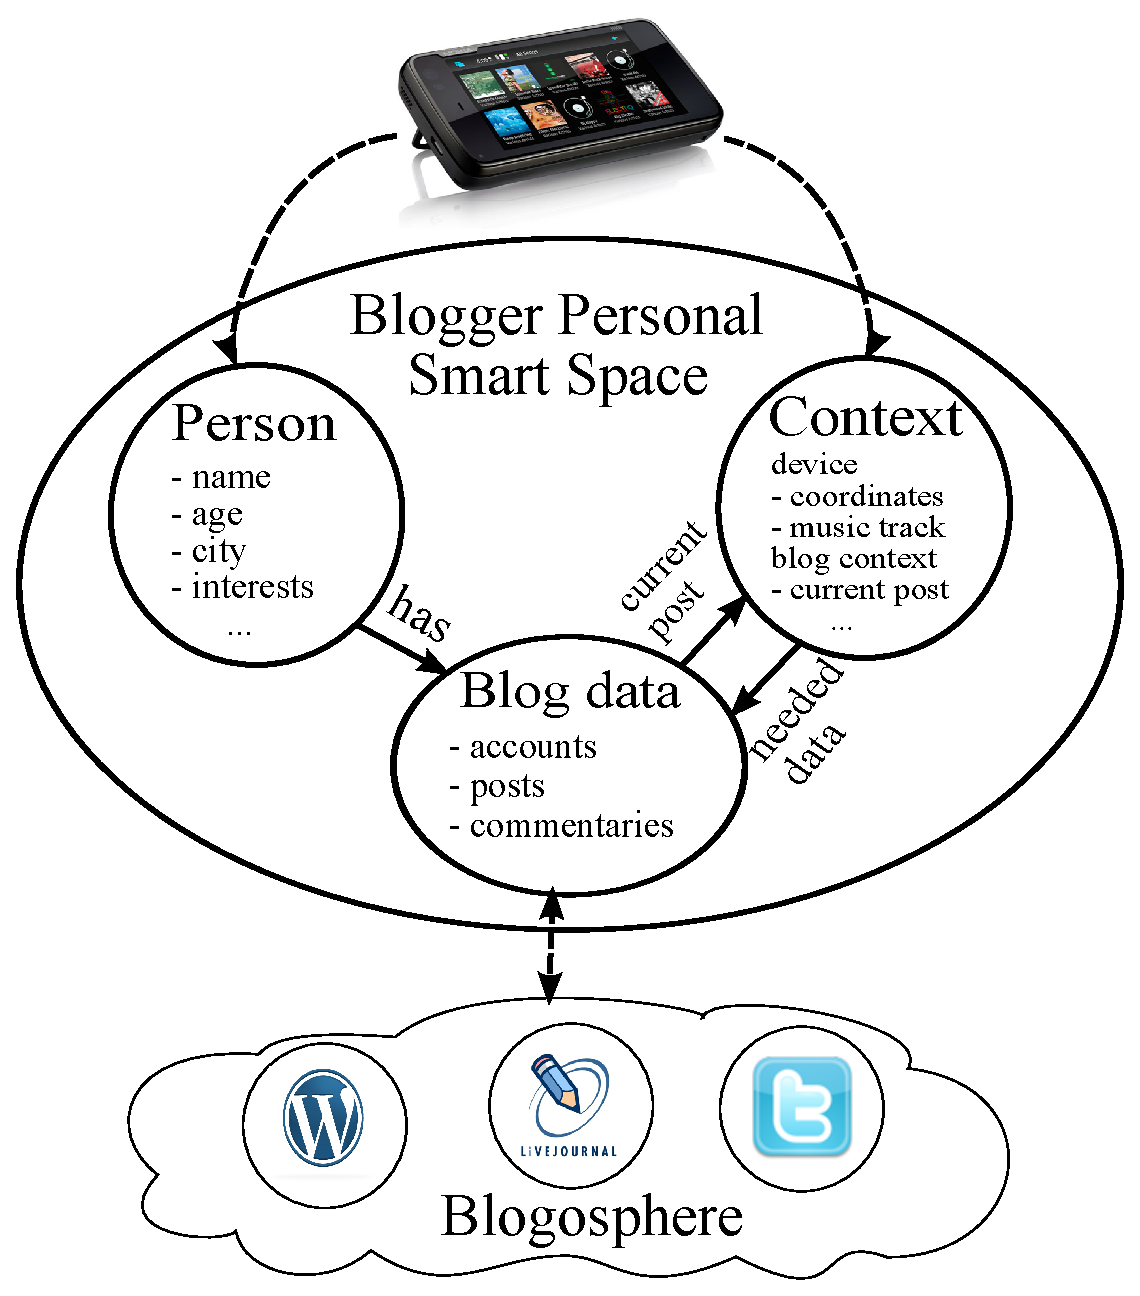
\epsfig{file=images/Personal-struct.eps, width=10cm}}
\caption{Структура персонального пространства блоггера}
\label{personal-struct}
\end{figure}

Знания, хранимые в персональном пространстве, можно разделить на три класса: 1) персональные данные (Person); 2) контекстная информация (Context); 3)~блог данные (Blog data).

Персональные данные содержат постоянную или долговременную информацию (которая изменяется через продолжительный промежуток времени) о пользователе. В качестве примера можно привести такие данные как имя, фамилия, возраст, дата рождения, место проживания, адрес электронной почты, интересы и др.
Данная информация не связана и не зависит от блог данных или блогосферы и, следовательно, может быть использована другими интеллектуальными приложениями.

Контекстные данные содержат текущие или часто изменяемые характеристики пользователя, такие как текущее местоположение (координаты мобильного устройства), погода в текущей местности, музыкальный трек, прослушиваемый в данный момент, настроение пользователя. Кроме того контекст может хранить информацию и о блогах, например пост, который читает пользователь в данный момент. Контекстная информация может быть использована агентами медиаторами для осуществления рекомендаций пользователю.

Блог данные содержат информацию о всех аккаунтах пользователя на различных блог-сервисах, постах на каждом аккаунте и комментариях к постам. В ИП одновременно могут находиться не все
данные из блогосферы, а только та информация, которая будет необходима пользователю в ближайшее время.

Следует отметить, что перечисленные классы знаний могут быть связаны между собой. Например персональная информация может содержать данные о том, что у пользователя есть несколько аккаунтов на блог-сервисах и, соответственно, образуется связь между персональными и блог данными. Кроме того блог данные, в свою очередь, могут влиять на контекстную информацию, отражая в ней, например, читаемый в данный момент пост или блог.

Пример содержимого персонального пространства блоггера представлен в табл. \ref{tspace1} и \ref{tspace2}. Блог-данные состоят из объектов: аккаунтов, постов и комментариев, и каждый из них обладает собственными свойствами. В случае, если пользователь Alice решит изменить, например, заголовок своего поста (post-1), то в персональном пространстве значение свойства заголовка поста (title) будет изменено.

\begin{table}[h]
%\begin{flushleft}
\caption{Пример персональных данных и контекста пространства}
%\end{flushleft}
\begin{center}
\begin{tabular}{|c|l|l|}
\hline
{\bf Class} & \multicolumn{1}{|c|}{\bf Property} & \multicolumn{1}{|c|}{\bf Value} \\
\hline
\multirow{5}{*}{Person} & name & Alice \\
\cline{2-3}
& age & 20 \\
\cline{2-3}
& city & Petrozavodsk \\
\cline{2-3}
& account & account1 \\
\cline{2-3}
& ... & ... \\
\hline
\multirow{3}{*}{Context} & coordinates & 61.7;34.2 \\
\cline{2-3}
& track & Mozart -- Lacrimosa \\
\cline{2-3}
& ... & ... \\
\hline
\end{tabular}

\label{tspace1}
\end{center}
\end{table}


\begin{table}[h]
\caption{Пример блог-данных пространства}
\begin{center}
\begin{tabular}{|l|l|l|}
\hline
\multicolumn{3}{|c|}{\bf Blog data} \\
\hline
\multicolumn{1}{|c|}{\bf Blog object} & \multicolumn{1}{|c|}{\bf Property} & \multicolumn{1}{|c|}{\bf Value} \\
\hline
account-1 & hasPost & post-1 \\
\hline
post-1 & title & My journey \\
\hline
post-1 & text & My journey was so wonderful! \\
\hline
\end{tabular}
\end{center}
\label{tspace2}
\end{table}
\newpage
Персональные пространства блоггеров могут взаимодействовать друг с другом и образовывать композицию. Существует несколько способов организации взаимодействия между пользовательскими пространствами.

{\bf 1. Дублирование данных}.
В данном случае при взаимодействии с другим пользовательским пространством, необходимые данные копируются в пользовательское пространство через блог-процессор. Такой способ используется если пользователь, данные которого получаются, не пользуется SmartScribo и данные а его аккаунте, постах и комментариях сохраняются в персональном пространстве текущего пользователя. Однако в случае, если такой пользователь будет иметь своё персональное пространство в ИП, то его данные будут продублированы.

{\bf 2. Установление связи}.
Композиция заключается в установлении связей между знаниями из разных пользовательских пространств. Примером композиции может быть отражение дружеских отношений на блог-сервисах между двумя пользователями SmartScribo (рис. \ref{personal-spaces}). 
Если аккаунты обоих пользователей являются друзьями на блог-сервисе, то в ИП можно определить связь <<Friend>> между этими аккаунтами, и в дальнейшем для получения информации блоггером о его друге достаточно будет обратиться в дружеское персональное пространство, минуя обращение к блог-сервису.

{\bf 3. Использование агента-посредника}.
При использовании данного подхода агент, работающий с конкретным персональным пространством получает данные из другого персонального пространства через специальный агент посредник. Одним из способов реализации данного подхода является механизм нотификаций, который будет расписан подробнее далее.

\begin{figure}[h]
\centerline{
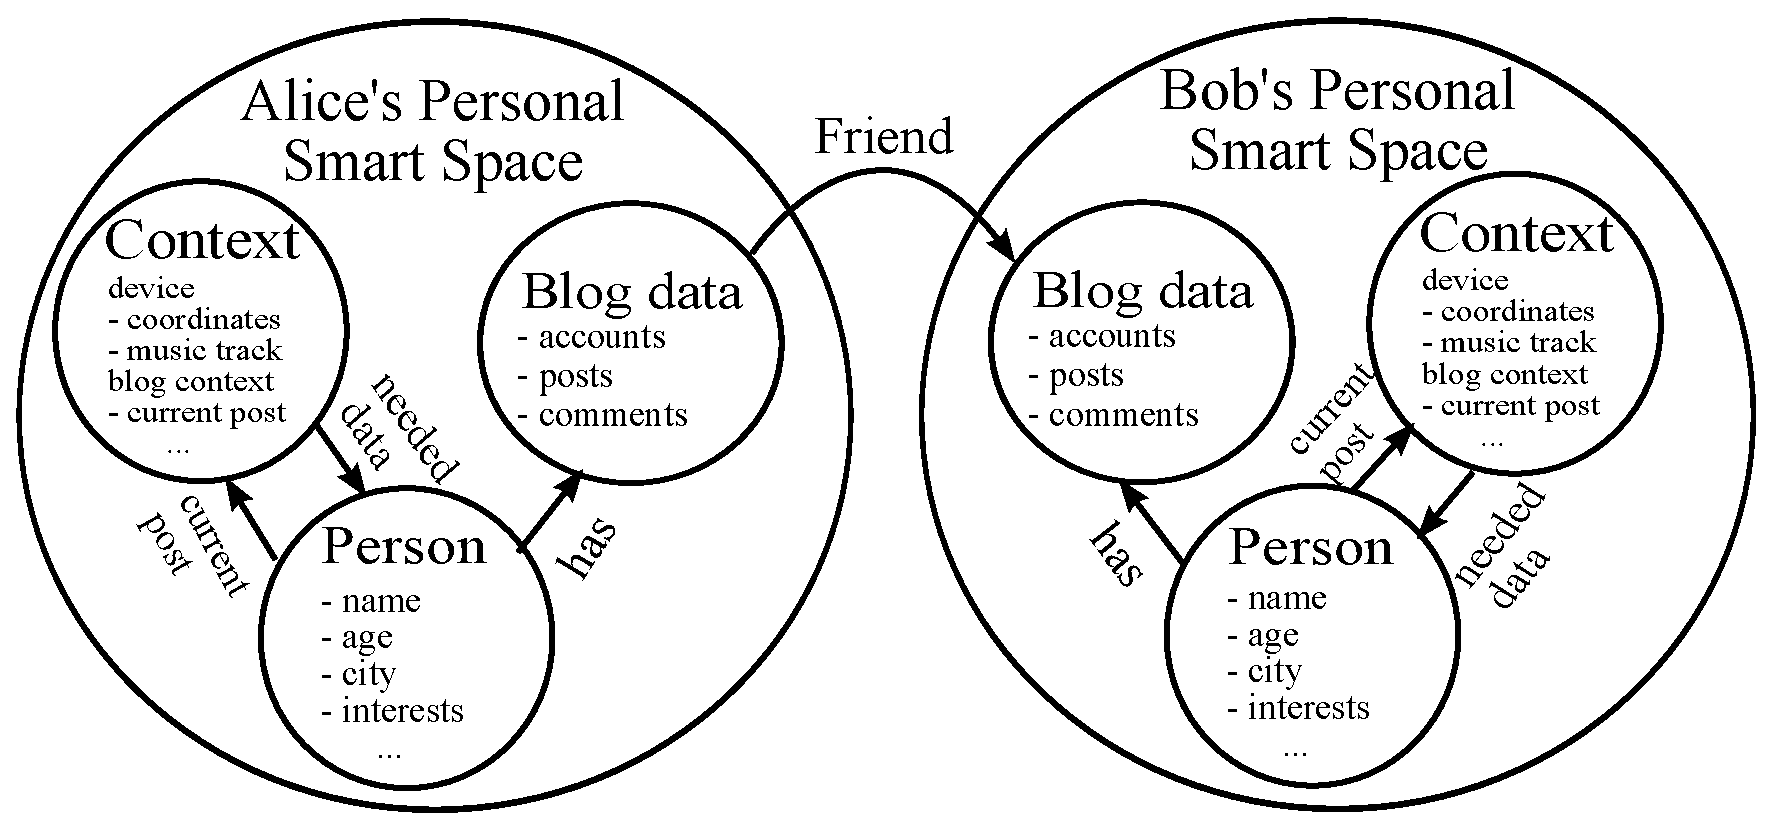
\epsfig{file=images/Scribo-spaces.eps, width=16cm}}
\caption{Композиция персональных пространств}
\label{personal-spaces}
\end{figure}

Персональное пространство блоггера содержит структурированную информацию о пользователе, его контексте и блог-данных. Для того чтобы использовать пространство в интеллектуальном приложении, необходимо описать его онтологическое представление.

\section{Онтологическая модель блогосферы}

В соответствии с устройством программной платформы Smart-M3 все знания, хранящиеся в ИП, представлются в виде RDF-триплетов. Совокупность RDF-триплетов, описывающих предметную область, образует онтологию, которая может быть представлена в виде классов и свойств. Следовательно для представления и хранения данных персонального пространства, включающих блогосферу, необходимо описать онтологию.

Для онтологического представления персонального пространства блоггера за основу была взята стандартная спецификация FOAF \cite{foaf}. Она определена как словарь именованных классов и свойств с использованием технологий RDF и OWL. FOAF позволяет описывать некоторые основные данные о пользователе, отношения между пользователями, а также наличие аккаунтов на некоторых сервисах. Профили FOAF могут быть использованы для поиска других людей со схожими характеристиками.

Однако FOAF не позволяет описывать непосредственно содержимое блог-аккаунтов, и следовательно возникает необходимость расширения данной онтологии для представления блог данных. Использование стандартных онтологий является одним из основных принципов онтологического моделирования, так как позволяет унифицировать фрагменты общей онтологии, вследствие чего другим разработчикам будет проще работать с новой онтологией. Онтология, используемая в SmartScribo, изображена на рис.~\ref{ont-tree}. Данная онтология описана в терминах OWL классов и их свойств.
\begin{figure}[h]
\centerline{
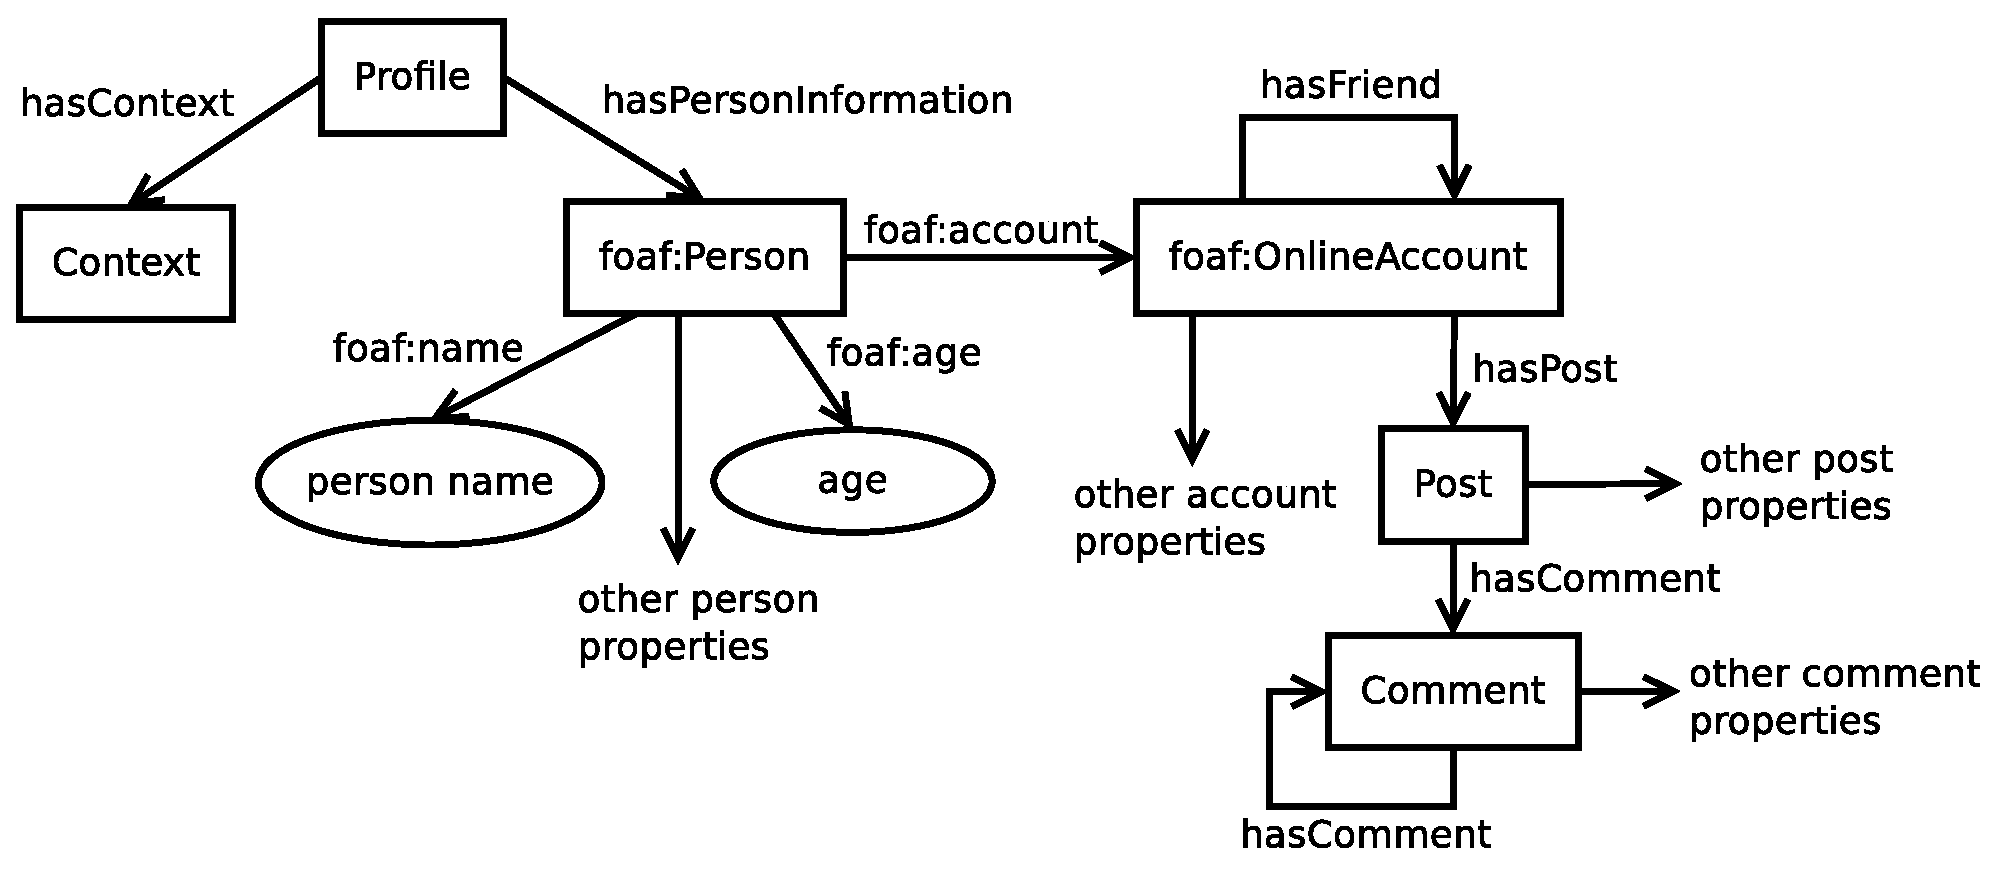
\epsfig{file=images/smartscribo-tree.eps, width=16cm}}
\caption{Онтология SmartScribo}
\label{ont-tree}
\end{figure}

Корнем онтологического дерева является класс {\tt Profile}, хранящий в себе остальную структуру знаний персонального пространства и блогосферы. Каждый экземпляр данного класса соответствует только одному пользователю или пользовательскому устройству и имеет свой уникальный идентификатор. Класс связан с персональной информацией о пользователе через свойство <<hasPersonInformation>> и с контекстными данными через свойство <<hasContext>>.
В формате OWL описание данного класса и связь его с классом FOAF имеет следующий вид:

{\small
\begin{verbatim}
<!-- Описание класса Profile -->
<owl:Class rdf:ID="Profile"/>

<!-- Описание свойства-связи personInformation 
     между классами Profile и foaf:Person -->
<owl:ObjectProperty rdf:ID="personInformation">
  <rdfs:domain rdf:resource="#Profile"/>
  <rdfs:range rdf:resource="http://xmlns.com/foaf/0.1/Person"/>
</owl:ObjectProperty>
\end{verbatim}
}
Тег {\tt owl:ObjectProperty} определяет объектное свойство (связь) между двумя классами, где тег {\tt rdfs:domain} --- это класс, обладающий данным свойством, а {\tt rdfs:range} --- тип значения свойства (в объектном свойстве тип значения должен быть другим классом). Ссылка на класс или свойство осуществляется при помощи атрибута {\tt rdf:resource}.

Класс {\tt Context} содержит частоизменяемую и временную контекстную информацию пользователя. Все знания, хранящиеся в этом классе преимущественно имеют текстовый вид, например текущие координаты, имя музыкального трека, настроение пользователя. Однако класс контекстной информации может содержать и ссылки на другие области знаний онтологии, такие как ссылка на пост из блог-данных, читаемый пользователем в данный момент. Контекстные данные выделены в отдельный класс, вследствие того, что множество интеллектуальных агентов могут получать или изменять контекст пользователя. Данный класс расположен на втором уровне иерархии классов в онтологии, поэтому другие агенты могут быстро получить доступ к этим данным, зная только идентификатор профиля пользователя.

Класс {\tt foaf:Person}, взятый из спецификации FOAF, содержит постоянные или редко-меняющиеся характеристики пользователя. В онтологии SmartScribo используются следующие свойства FOAF: имя пользователя (<<foaf:name>>), возраст (<<foaf:age>>), дата рождения (<<foaf:birthday>>), адрес электронной почты (<<foaf:mbox>>). Эти данные вместе с контекстом могут быть использованы агентами-медиаторами SmartScribo для предоставления рекомендаций пользователю. Кроме этого класс {\tt foaf:Person} обладает свойством <<foaf:account>>, которое связывает пользовательскую информацию с классом {\tt foaf:OnlineAccount}, содержащим данные об аккаунтах пользователя. Таким образом через указанное свойство связаны персональная информация и блог-данные.

Класс {\tt foaf:OnlineAccount} представляет собой класс FOAF, описывающий конкретную учётную запись на некотором сервисе. Свойство <<foaf:Name>> описывает имя аккаунта. В онтологии SmartScribo данный класс расширяется набором дополнительных свойств: <<login>> -- логин пользовательского аккаунта, <<password>> -- пароль учётной записи для осуществления авторизации на сервисе блог-процессором (в ИП хранится в зашифрованном виде), <<userpic>> -- ссылка до изображения иконки пользователя на сервисе, <<bdate>> -- дата рождения, указанная пользователем на сервисе, <<groupname>> -- группа в которой состоит данный аккаунт. Кроме этого аккаунт обладает свойством <<hasPost>>, связывающим этот аккаунт с индивидами класса {\tt Post}, т.е. со всеми постами указанной учётной записи. На языке OWL расширение класса {\tt foaf:OnlineAccount} осуществляется следующим образом:

{\small
\begin{verbatim}
<!-- Описание строкового свойства bdate
     у класса foaf:OnlineAccount -->
<owl:DatatypeProperty rdf:ID="bdate">
  <rdfs:domain rdf:resource="http://xmlns.com/foaf/0.1/OnlineAccount"/>
  <rdfs:range rdf:resource="http://www.w3.org/2001/XMLSchema#string"/>
</owl:DatatypeProperty>

<!-- Описание свойства-связи hasPost 
     между классами foaf:OnlineAccount и Post -->
<owl:ObjectProperty rdf:ID="hasPost">
  <rdfs:domain rdf:resource="http://xmlns.com/foaf/0.1/OnlineAccount"/>
  <rdfs:range rdf:resource="#Post"/>
</owl:ObjectProperty>
\end{verbatim}
}
Тег {\tt owl:DatatypeProperty} определяет свойство у класса, указанного в теге {\tt rdfs:domain}, с типом данных этого свойства, указанным в теге {\tt rdfs:range}.

Класс {\tt Post} содержит полную информацию о конкретном посте на определённом аккаунте блог-сервиса. Данный класс содержит свойства, отражающие основные характеристики поста: <<title>> -- заголовок поста, <<text>> -- текстовое содержимое поста, <<pdate>> -- дата создания или последнего изменения, <<tags>> -- тэги поста, <<journal>> -- необязательное свойство, содержащее имя группы, в которую был отправлен пост. В онтологическом представлении посты не являются упорядоченными, поэтому их упорядочивание по дате должно происходить на стороне получающего агента по свойству <<pdate>>. Класс {\tt Post} использует свойство <<hasComment>> для связи данного поста с комментариями.

Класс {\tt Comment} содержит данные, относящиеся к комментарию, и схож с классом {\tt Post}. Данный класс включает в себя свойства <<title>>, <<text>>, <<pdate>>, <<journal>>. Комментарий также обладает свойством <<hasComment>>, так как на блог-сервисах есть возможность отправки комментария на комментарий. Таким образом каждая блог-дискуссия, состоящая из поста и его комментариев, имеет древовидную структуру.

Пример онтологического представления персонального пространства блоггера изображён на рис.~\ref{ont-example}. В данном примере отражены данные из табл. \ref{tspace1} и \ref{tspace2}.
Прямоугольниками индивиды соответствующих классов: {\tt Profile}, {\tt foaf:Person}, {\tt Context}, {\tt foaf:Account}, {\tt Post}. Для удобства определения данных в ИП, имя индивида состоит из названия класса и уникального идентификатора, но фактически имя индивида может быть произвольным и уникальным. Овалами на изображении обозначены конкретные значения свойств индивидов. Если пользователь Alice решит изменить, например, заголовок своего поста (post-e87a25d1) на <<My weekend>>, то триплет <<post-e87a25d1, title, My journey>> будет заменён на триплет <<post-e87a25d1, title, My weekend>>.

\begin{figure}[h]
\centerline{
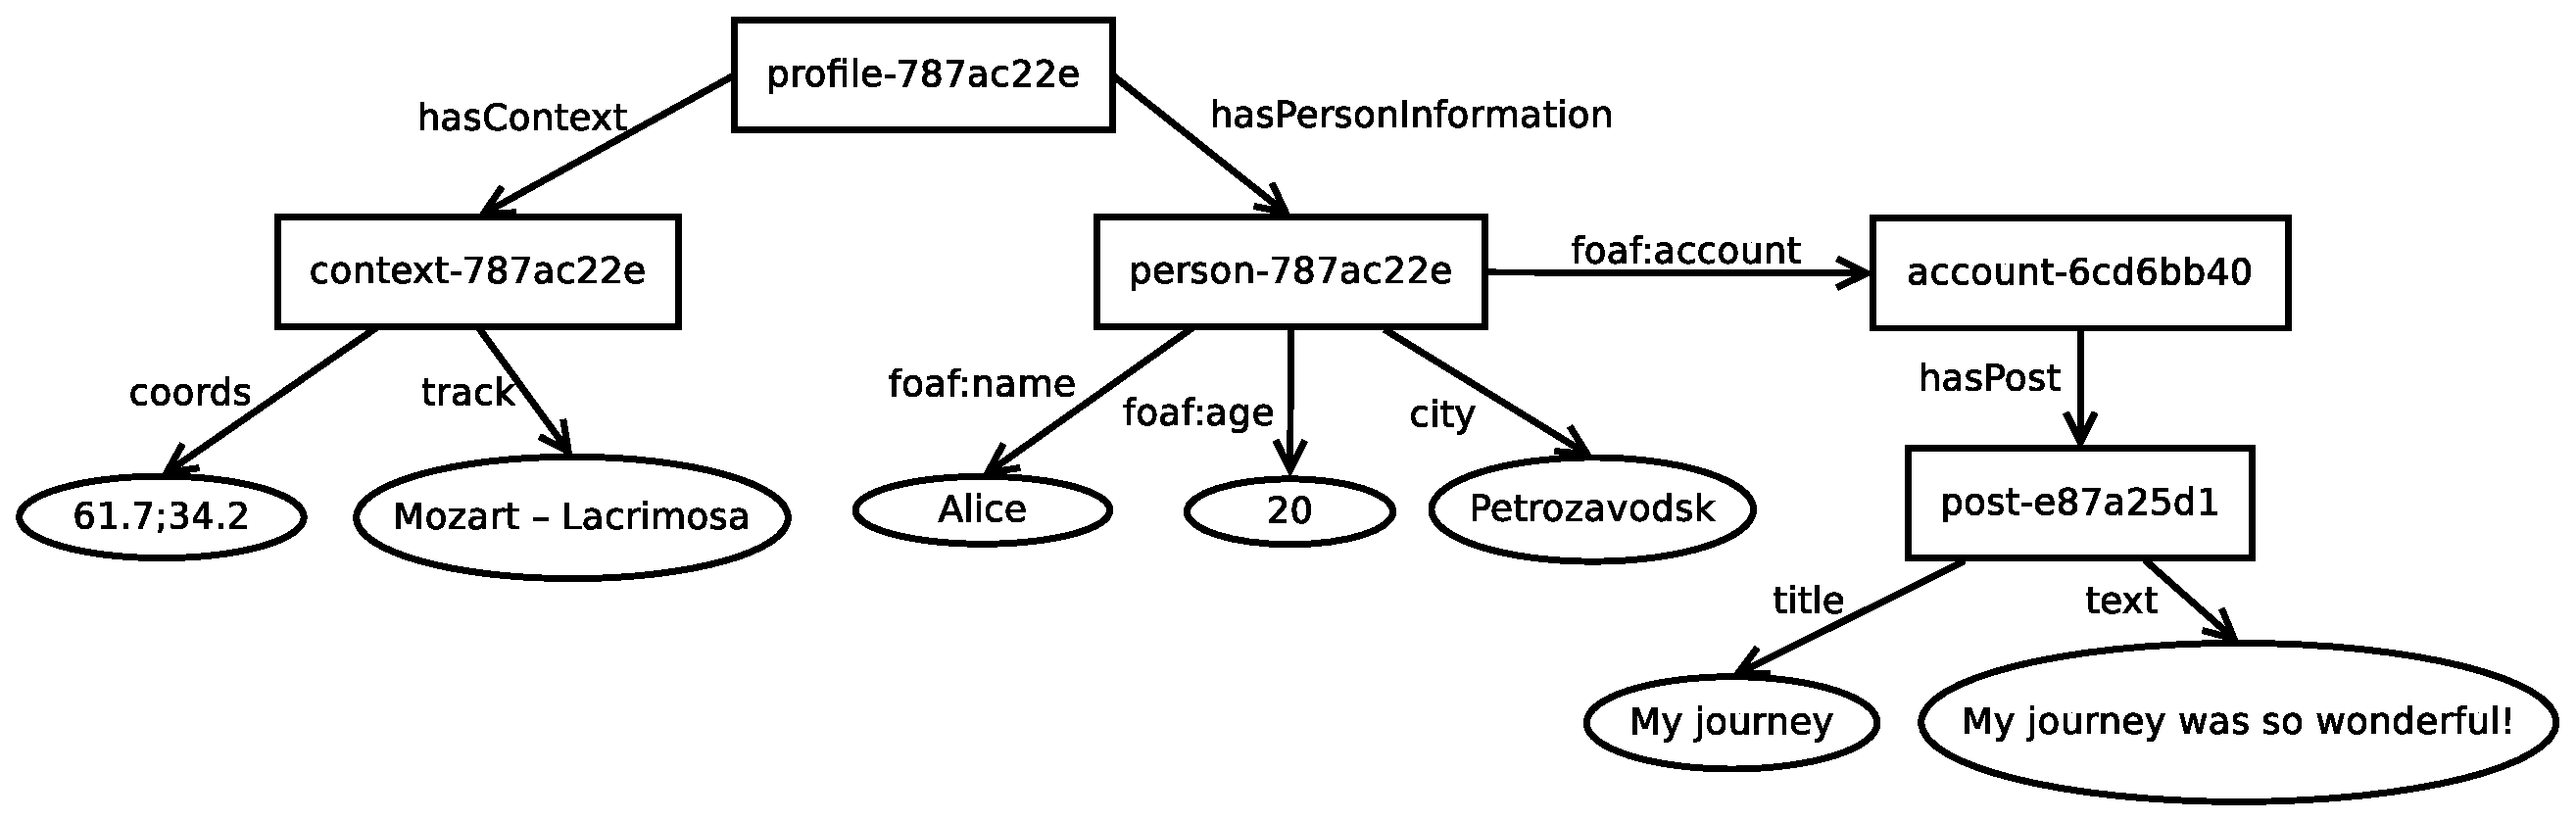
\epsfig{file=images/smartscribo-tree-example.eps, width=16cm}}
\caption{Пример онтологического представления пространства}
\label{ont-example}
\end{figure}

Стоит отметить, что для управления онтологическими данными блогосферы подписка на объекты онтологии не является эффективной, вследствие того, что даже на одном аккаунте для определения агентом изменений в посте или комментарии необходимо подписаться на большое количество триплетов (должны отслеживаться изменения всех свойств постов или комментариев). Отсюда следует, что необходимо создание более эффективного механизма, позволяющего определять изменения онтологических данных блогосферы.

\section{Модель нотификаций} 

Онтологические данные блогосферы состоят из множнества однотипных объектов, управление которыми является неэффективным при использовании подписки на их свойства, так как создаётся большое количество подписок и сложность их обработки возрастает. Кроме этого при существовании множества клиентов и блог-процессоров SmartScribo необходимы способы координации взаимодействия этих агентов. В данном разделе мы рассмотрим вариант решения упомянутых проблем --- модель нотификаций.

Модель нотификаций --- это онтологическая модель, предназначенная для координации взаимодействия между агентами SmartScribo. Нотификация инициирует соответствующего агента выполнить указанную операцию или сообщает о результате выполнения операции. Нотификация представляет собой триплет или набор триплетов, которые соответствуют выполнению действия или его результату.

Общая схема процесса нотификации, рассмотренная на примере взаимодействия клиентского агента и блог-процессора, изображена на рис. \ref{notification}.
\begin{figure}[h]
\centerline{
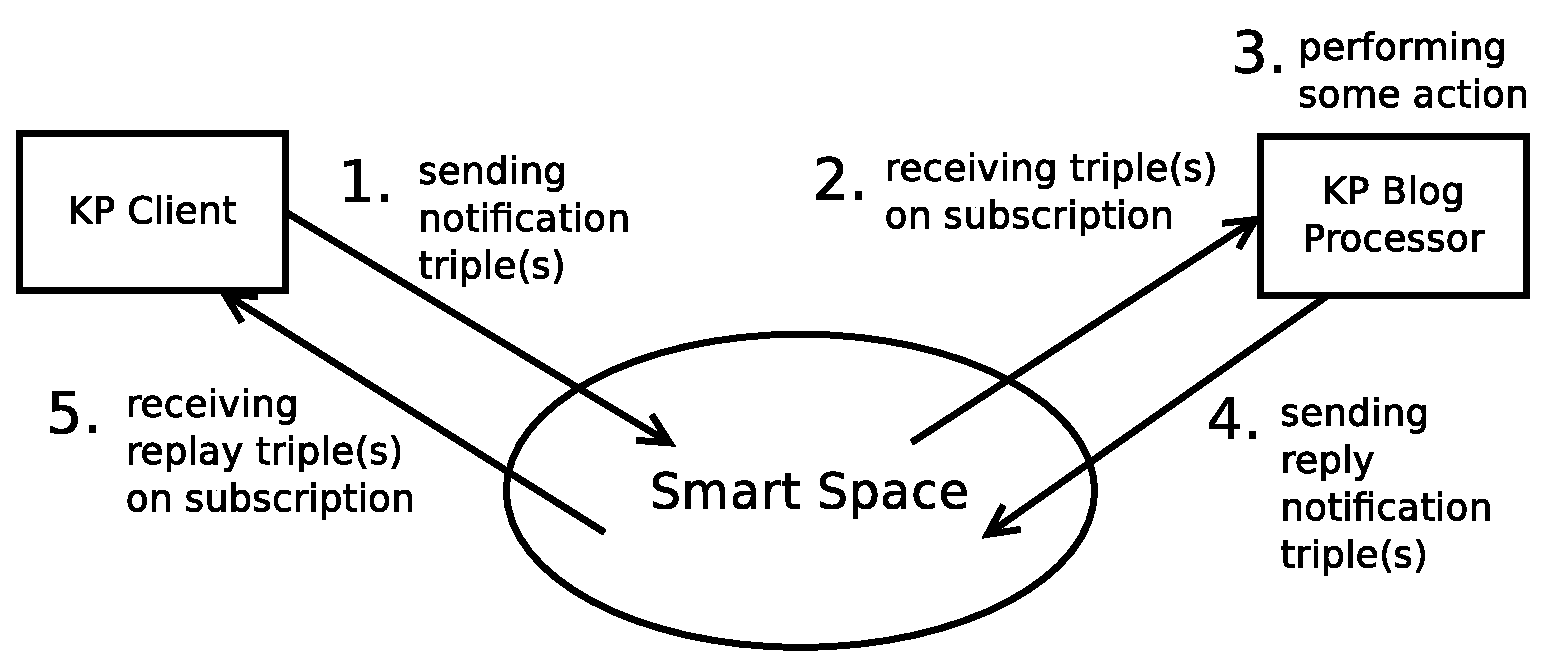
\epsfig{file=images/notifications.eps, width=12cm}}
\caption{Схема нотификации для двух агентов: клиента и блог-процессора}
\label{notification}
\end{figure}
Процесс нотификации состоит из пяти шагов.
\begin{enumerate}
\item
Клиентскому агенту необходимо инициировать выполнение требуемого действия у блог-процессора. Клиент публикует соответствующий триплет нотификации в ИП.
\item
Агент блог-процессор получает адресованную ему нотификацию вместе со всеми параметрами нотификации (получение происходит засчёт подписки на триплет нотификации).
\item
Агент-получатель выполняет необходимую операцию в соответствии с параметрами нотификации.
\item
Агент-получатель публикует в ИП ответную нотификацию с результатами выполнений действия.
\item
Клиентский агент получает ответную нотификацию, через механизм подписки. 
\end{enumerate}

Нотификации могут быть разделены на два типа в зависимости от момента их отправки и ожидания ответной нотификации агентом инициатором: реактивные и проактивные.

Реактивная нотификация инициирует у агента выполнение требуемой операции и высылается в зависимости от действия пользователя. Инициирующий агент ожидает ответной нотификации с результатом выполнения операции. Примером реактивной нотификации может быть нотификация проверки логина и пароля учётной записи или нотификация отправки поста на блог-сервис.

Проактивная нотификация высылается в фоновом режиме и только косвенным образом зависит от действий пользователя. Инициирующий агент чаще всего не ожидает ответной нотификации. В большинстве случаев проактивная нотификация влияет или зависит от контекстной информации пользователя. В качестве примера такой нотификации можно привести нотификацию, инициирующую поиск постов схожих по тематике с постом, читаемым в данный момент.

Модель нотификаций является надстройкой к онтологической модели блогосферы. В каждой нотификации чаще всего содержится связь с онтологическими данными, т.е. триплет нотификации указывает на индивида из онтологии блогосферы.

Нотификации могут быть простыми, состоящими из одного триплета, и сложными, представленными в виде цепочки триплетов. Простая нотификация используется в том случае, когда инициируемому агенту требуется передать только один параметр, необходимый для выполнения операции. Общий вид простой нотификации следующий:
$$
\mathrm{Notification} \mbox{<{\tt type}>}, \mbox{<{\tt action}>}, \mbox{<{\tt value}>}
$$
где {\tt type} содержит тип блог-процессора или идентификатор клиента, которому адресована нотификация, {\tt action} --- название действия которое должно быть выполнено или было выполнено (в ответной нотификации), а {\tt value} --- имя необходимого индивида в онтологии или результат выполнения действия. Все ответные нотификации являются простыми.

Сложная нотификация представляет собой цепочку триплетов и используется в случае, когда для выполнения действия необходимо передать несколько параметров. Общий вид сложной нотификации следующий:

$$
\begin{array}{l}
\mbox{Notification} \mbox{<{\tt type}>}, \mbox{<{\tt action}>}, \mbox{notif\_ind<{\tt id}>} \\
\mbox{notif\_ind<{\tt id}>}, \mbox{<{\tt parameter1}>}, \mbox{<{\tt value1}>}\\
\mbox{notif\_ind<{\tt id}>}, \mbox{<{\tt parameter2}>}, \mbox{<{\tt value2}>}\\
...
\end{array}
$$
где \mbox{notif\_ind<{\tt id}>} дополнительный индивид с идентификатором {\tt id}, хранящий все значения параметров нотификации, {\tt parameter} --- название параметра и {\tt value} --- значение этого параметра (ссылка на онтологические данные или строка).

Нотификации можно классифицировать по типу объекта над которым выполняется действие: %работа с аккаунтом, постами, комментариями и друзьями.

{\bf 1. Работа с аккаунтами}.
\vspace{-0.25cm}
\begin{list}{}{}
\item
Для работы с аккаунтами предназначена только одна нотификация, которая инициирует получение данных об аккаунте с блог-сервиса, а также проверку логина и пароля:

\mbox{Notification<{\tt service}>, refreshAccount, <{\tt acc\_id}>}

{\tt service} --- тип сервиса (LJ -- LiveJournal, TW -- Twitter, и т.д.)\\
{\tt acc\_id} --- ссылка на индивида необходимого аккаунта (идентификатор индивида)

ответная нотификация, возвращающая результат получения данных аккаунта и проверки логина и пароля, имеет следующий вид:

\mbox{Notification<{\tt client\_id}>, refreshAccount, ok/error}

{\tt client\_id} --- идентификатор индивида профиля пользователя (класс Profile)\\
Все ответные нотификации имеют аналогичный вид, поэтому далее они указываться не будут.
\end{list}

{\bf 2. Работа с постами}.
\begin{itemize}
\item обновление постов указанного аккаунта

\mbox{Notification<{\tt service}>, refreshPosts, <{\tt acc\_id}>}

\item отправка поста в собственный блог или в группу

\mbox{Notification<{\tt service}>, sendPost, post\_notif<{\tt id}>}\\
\mbox{post\_notif<{\tt id}>, postAcc, <{\tt acc\_id}>}\\
\mbox{post\_notif<{\tt id}>, postId, <{\tt post\_id}>}\\
\mbox{post\_notif<{\tt id}>, journal, <{\tt journal\_name}>}

свойство <<postAcc>> хранит ссылку на индивида аккаунта {\tt acc\_id}, от имени которого будет послан пост\\
свойство <<postId>> хранит ссылку на индивида поста {\tt post\_id}, данные которого будут посланы на блог-сервис\\
свойство <<journal>> хранит название группы в которую будет опубликован пост (таких триплетов может быть несколько)

\item редактирование

\mbox{Notification<{\tt service}>, editPost, post\_notif<{\tt id}>}\\
\mbox{post\_notif<{\tt id}>, oldPost, <{\tt post1\_id}>}\\
\mbox{post\_notif<{\tt id}>, newPost, <{\tt post2\_id}>}

Пост с идентификатором {\tt post1\_id} будет отредактирован на блог-сервисе в соответствии с данными пости с идентификатором {\tt post2\_id}. В ИП старый пост будет удалён, а отредактированный пост будет связан с аккаунтом.

\item удаление


\mbox{Notification<{\tt service}>, delPost, post\_notif<{\tt id}>}\\
\mbox{post\_notif<{\tt id}>, postAcc, <{\tt acc\_id}>}\\
\mbox{post\_notif<{\tt id}>, postId, <{\tt post\_id}>}\\
\mbox{post\_notif<{\tt id}>, journal, <{\tt journal\_name}>}

Удаляется пост, имеющий идентификатор {\tt post\_id}, с указанного аккаунта {\tt acc\_id}, а также из групп {\tt journal\_name}

\end{itemize}

{\bf 3. Работа с комментариями}.

\begin{itemize}
\item обновление комментариев указанного аккаунта

\mbox{Notification<{\tt service}>, refreshComments, <{\tt acc\_id}>}

\item отправка

\mbox{Notification<{\tt service}>, sendComment, com\_notif<{\tt id}>}\\
\mbox{com\_notif<{\tt id}>, comAcc, <{\tt acc\_id}>}\\
\mbox{com\_notif<{\tt id}>, comId, <{\tt com\_id}>}\\
\mbox{com\_notif<{\tt id}>, parId, <{\tt parrent\_id}>}\\
\mbox{com\_notif<{\tt id}>, journal, <{\tt journal\_name}>}

Отправка комментария, имеющего идентификатор {\tt com\_id}, от имени пользователя аккаунта {\tt acc\_id}. Комментарий отправляется на пост или другой комментарий с идентификатором {\tt parrent\_id}, либо в группу {\tt journal\_name}.

\item удаление

\mbox{Notification<{\tt service}>, delComment, com\_notif<{\tt id}>}\\
\mbox{com\_notif<{\tt id}>, comAcc, <{\tt acc\_id}>}\\
\mbox{com\_notif<{\tt id}>, comId, <{\tt com\_id}>}\\
\mbox{com\_notif<{\tt id}>, parId, <{\tt parrent\_id}>}\\
\mbox{com\_notif<{\tt id}>, journal, <{\tt journal\_name}>}

Удаление комментария, имеющего идентификатор {\tt com\_id}, от имени пользователя аккаунта {\tt acc\_id}. Комментарий удаляется у пост или другого комментария с идентификатором {\tt parrent\_id}, либо в группе {\tt journal\_name}.

\end{itemize}
\newpage
{\bf 4. Работа с друзьями}.

\begin{itemize}
\item
добавление пользователя в друзья

\mbox{Notification<{\tt service}>, addFriend, friend\_notif<{\tt id}>}\\
\mbox{friend\_notif<{\tt id}>, ownAcc, <{\tt acc\_id}>}\\
\mbox{friend\_notif<{\tt id}>, friendName, <{\tt name}>}

Добавление в аккаунт {\tt acc\_id} пользователя с именем {\tt name}.

\item
удаление пользователя из друзей

\mbox{Notification<{\tt service}>, delFriend, friend\_notif<{\tt id}>}\\
\mbox{friend\_notif<{\tt id}>, ownAcc, <{\tt acc\_id}>}\\
\mbox{friend\_notif<{\tt id}>, friendName, <{\tt name}>}

Удаление пользователя с именем {\tt name} у аккаунт {\tt acc\_id}.

\item
обновление списка друзей

\mbox{Notification<{\tt service}>, refreshFriends, <{\tt acc\_id}>}

\item
обновление данных о постах друзей

\mbox{Notification<{\tt service}>, refreshFriendsPosts, <{\tt acc\_id}>}

\end{itemize}

\begin{figure}[h]
\centerline{
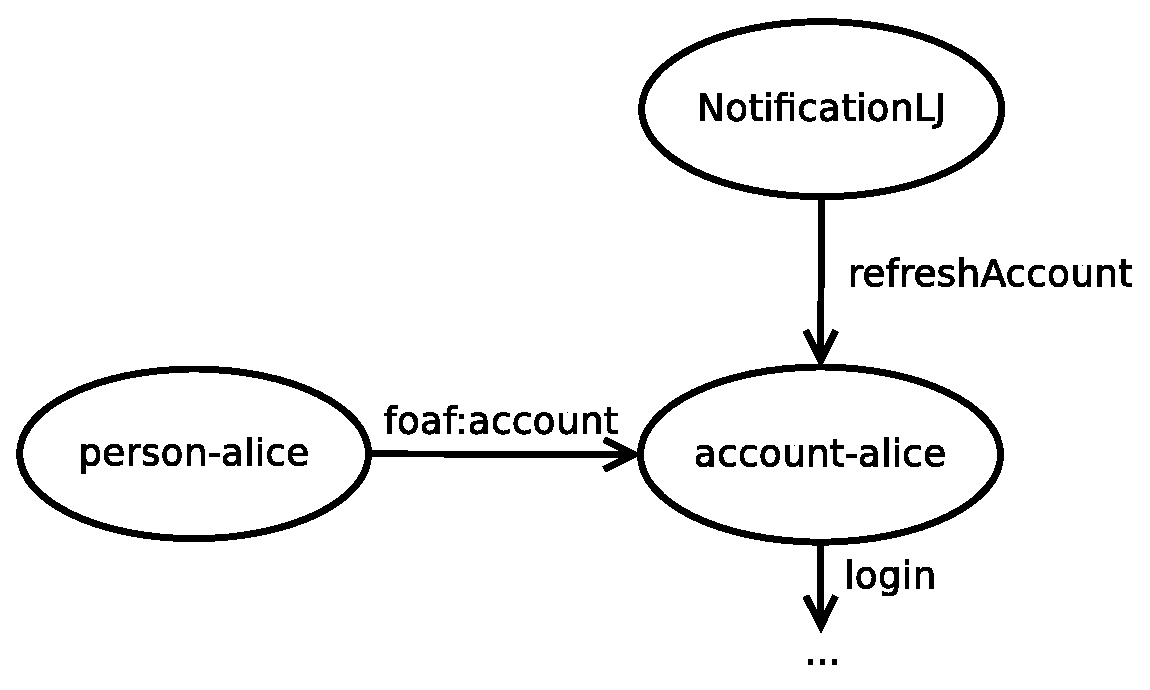
\epsfig{file=images/notifications-example.eps, width=10cm}}
\caption{Пример нотификации}
\label{notification-example}
\end{figure}

Пример использования нотификации представлен на рис. \ref{notification-example}.
Пользователь Alice обладает аккаунтом на блог-сервисе LiveJournal. Информация о пользователе и аккаунте хранится в персональном пространстве в ИП у индивидом с идетификаторами <<person-alice>> и <<account-alice>> соответственно. Для синхронизации данных об аккаунте, а также проверки указанного логина/пароля клиентский агент Alice высылает нотификацию вида <<NotificationLJ, refreshAccount, account-alice>>. Блог-процессор, взаимодействующий с LiveJournal, получает данную нотификацию и зная идентификатор индивида аккаунта Alice (объект в триплете), получает возможность обратиться к свойствам аккаунта (логин, пароль, и т.д.) и выполнить соответствующую операцию.

Таким образом нотификации являются удобным механизмом управления онтологическими данными, позволяющим обрабатывать информацию, разделять подписки агентов на триплеты (каждый агент получает нотификации, адресованные только ему), а также синхронизировать взаимодействия между агентами.

\section{Реализация блог-процессора}

В данном разделе будет рассмотрена работа с онтологическими данными на стороне блог-процессора.

Архитектура блог-процессора представлена на рис. \ref{arch-bp}. В блог-процессоре можно выделить две основных подсистемы: подсистема взаимодействия с блог-сервисом (Blog service connector) и подсистема взаимодействия с ИП (Smart-M3 Node).

\begin{figure}[h]
\centerline{
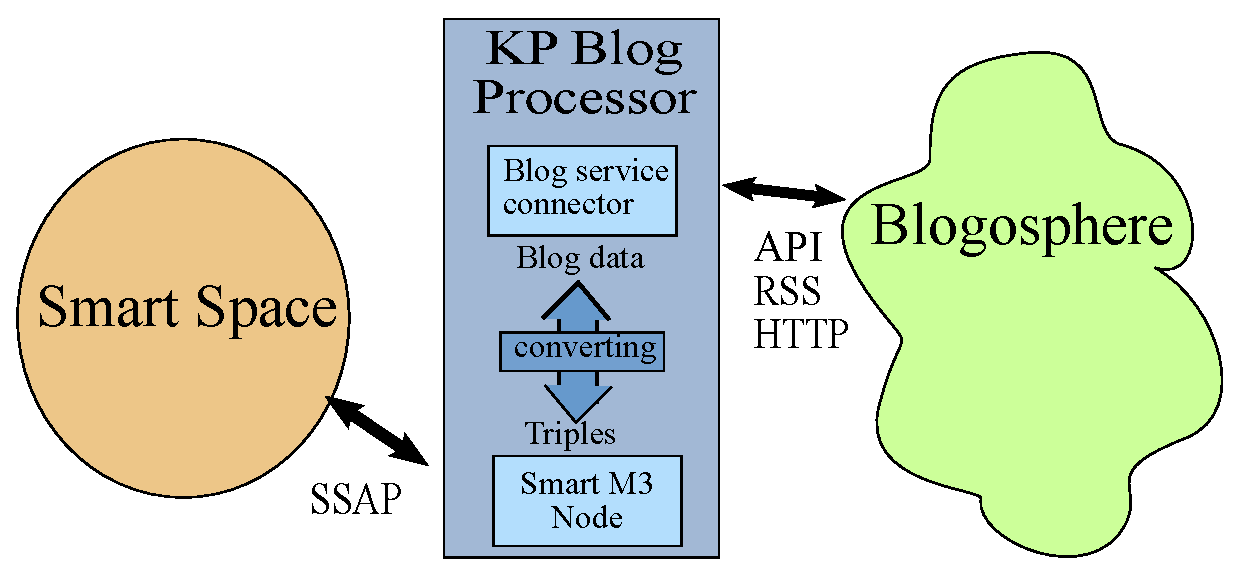
\epsfig{file=images/arch_kp_bp.eps, width=14cm}}
\caption{Архитектура блог-процессора}
\label{arch-bp}
\end{figure}

Подсистема взаимодействия с блог-сервисом должна осуществлять следующие функции:
\begin{itemize}
\item авторизация на сервисе
\item получение информации о пользователе (профиль + списки друзей)
\item получение постов для указанного аккаунта
\item отправка/изменение/удаление постов
\item получение комментариев для указанного аккаунта
\item отправка/удаление комментариев
\item добавление/удаление друзей
\end{itemize}

Существует несколько способов взаимодействия с блог-сервисом, каждый из которых обладает своими преимуществами и недостатками.

{\bf 1. Использование API блог-сервиса}.
Многие блог-сервисы предоставляют API для взаимодействия с ними. API явлется удобным способом взаимодействия с сервисом и позволяет получать данные в каком-либо популярном формате. Например LiveJournal предоставляет возможность взаимодействия по протоколу XML-RPC и получения данных в XML формате, который прост в обработке. API позволяет как получать блог-данные с сервиса, так и отправлять их на сервис, однако данный способ взаимодействия не всегда предоставляет все необходимые функции для блоггинга (например на некоторых сервисах нет возможности работы с комментариями) и для работы обязательно необходима авторизация пользователя.

{\bf 2. Использование RSS}.
RSS позволяет получать основные данные с блог-сервиса не требуя авторизации пользователя. Данные полученные с помощью RSS также представлены в формате XML и легко могут быть обработаны. Несмотря на это возможности RSS весьма ограничены, так как многие данные невозможно получить с помощью этого способа взаимодействия (возможно получение только фиксированное количество последних добавленных постов, комментарии не поддерживаются). Кроме этого при использовании RSS возможно только получение данных.

{\bf 3. Использование HTTP запросов}. 
Наиболее сложным способом взаимодействия с блог-сервисом является использование HTTP запросов. Данный подход эмулирует работу веб-браузера и, соответственно, позволяет использовать все возможности блог-сервиса. Однако реализация этого способа взаимодействия трудоёмка в связи с тем, что необходимо определять, какие запросы следует отправлять на сервер, а также производить разбор HTML страниц.

%ADD как в SmartScribo и специфика API

Подсистема взаимодействия с ИП получает данные от подсистемы взаимодействия с блог-сервисом и преобразует их в триплеты, соединяется с SIB, используя протокол SSAP, и осуществляет обработку онтологических данных (публикация, получение, подписка).

В общем случае существует несколько способов обработки онтологических данных агентами. Они различаются способом представления локальных данных в агенте. Основными моделями представления данных являются онтологическая и ОО модели.

{\bf 1. Онтологическая модель}.
При использовании онтологической модели представления, данные хранятся в локальной памяти агента в виде графа из RDF-триплетов, схожим с RDF-графом ИП. Некоторые блог-сервисы работают с онтологическим представлением данных, например Yandex предоставляет возможность взаимодействия с блогом с использованием спецификации FOAF.

Преимущества данного подхода заключаются в том, что в локальной памяти хранится структура данных совпадающая с ИП. При работе с локальной копией данных, появляется возможность использования специализированных средств обработки, таких как язык SPARQL для построения сложных запросов. Локальные онтологические данные также могут быть обработаны с помощью и других сторонних приложений. При использовании онтологического представления данных появляется возможность за один запрос получить большой объем данных и далее работать с ними локально, что уменьшит количество взаимодействий с ИП. 

Недостатком онтологического представления является требование к частой синхронизации локальных данных с ИП. При любом изменении в локальной копии данных, необходимо отражать эти изменения в ИП, так как это может повлиять на работу других интеллектуальных агентов. Также работа с онтологическими данными не всегда является простой и может потребовать применения или разработки специальных алгоритмов обработки информации.

{\bf 2. Объектно-ориентированная модель}.
Представление данных заключается в преобразовании полученных из ИП RDF-триплетов в объекты, хранящиеся в локальной памяти агента. При необходимости публикации данных в ИП, объект обратно преобразуется в триплеты.

Данный подход позволяет для каждого класса определить конкретные функции, используемые в определённых сценариях. При работе с данными проще осуществлять обработку объектов, чем RDF-графа. Примером может являтся работа с постами блога, которые преобразованы в объекты. Вследствие этого, несложно будет отсортировать все посты по дате в массиве постов-объектов.

Такой подход к представлению данных позволяет работать с объектом, как с выделенным фрагментом онтологии. В данном случае легко определить, какой фрагмент онтологических данных будет модифицирован, и отразить эти изменения в ИП. Преобразование RDF-триплетов в объекты также даёт возможность взаимодействия с сервисом посредством специализированных библиотек, таких как QMF. Такой подход будет разумным, если в QMF появятся плагины для соответствующих блог-сервисов.

Однако постоянное преобразование из триплетов в объекты и обратно приводит к дополнительным расходам ресурсов устройства, а также частому взаимодействию с ИП.

\vspace{0,5cm}

При разработке клиентского агента SmartScribo использовалась ОО-модель представления данных. Таким образом в памяти агента хранятся объекты, соответствующие аккаунтам пользователя, а также постам и комментариям в блогах. Данный подход позволяет осуществлять упорядочивание, сортировку, фильтрацию постов и комментариев, а также объединение всех блогов пользователя в один единый виртуальный блог.

В реализации агента блог-процессора применяется частный случай ОО-модели представления данных. Блог-процессору не требуется долгое время хранить в памяти данные об аккаунтах, постах, комментариях, так как он является транзитным. Блог-процессор получает структуры данных от библиотеки, взаимодействующей с блог-сервисом, преобразует их в триплеты и публикует в ИП, и аналогично в обратном направлении из ИП на блог-сервис. При таком способе работы не требуется хранить структуры данных в памяти и осуществлять их обработку. Так как один блог-процессор может обрабатывать запросы от нескольких клиентов, то при каждом запросе ему приходится получать из ИП данные авторизации пользователя, что увеличивает количество обращений к ИП. Вариантом улучшения представленной схемы работы является постоянное хранение в памяти агента некоторых пользовательских данных, содержащих данные авторизации и другие часто используемые данные.

Процесс функционирования блог-процессора схож с работой сервера. Блог-процессор ждёт получения нотификации от клиента, которая приходит благодаря механизму подписки, обрабатывает нотификацию и выполняет необходимые операции. Такое поведение пресуще агенту на протяжении всего времени его работы. Однако в качестве улучшения агента возможно также периодическое обновления некоторых блог-данных в ИП через определённый промежуток времени.

Одним из важных моментов реализации блог-процессора является организация подписки на триплеты нотификации. Возможны два способа подписки на нотификации: 
\begin{enumerate}
\item одна подписка на все виды нотификаций
\item отдельная подписка на каждое требуемое действие
\end{enumerate}

При использовании одной подписки на все виды нотификации блог-процессор подписывается на триплет вида:
$$
\mathrm{Notification} \mbox{<{\tt type}>}, \mbox{\tt ANY}, \mbox{\tt ANY}
$$
где {\tt type} --- это тип сервиса с которым взаимодействует блог-процессор, а {\tt ANY} --- шаблон в триплете, обозначающий что вместо него может находиться любое значение. При таком виде подписки все нотификации, пришедшие блог-процессору, будут обрабатываться последовательно, что может привести к длительному ожиданию при одновременной работе нескольких агентов. 

В случае использования отдельной подписки на каждую операцию, в агенте создаётся несколько обработчиков подписок на триплеты вида:
$$
\mathrm{Notification} \mbox{<{\tt type}>}, \mbox{<{\tt action}>}, \mbox{\tt ANY}
$$
где {\tt action} --- это название операции которую необходимо выполнить блог-процессору. В агенте создаётся такое количество подписок на указанные триплеты, сколько различных операций используется в модели нотификаций. Каждая подписка запускается в отдельном потоке, поэтому несколько разных операций могут выполняться параллельно. В связи с этим время ожидания клиентского агента до выполнения операции снижается. 

Несмотря на это в ситуациях, когда важна последовательность выполнения операций из нотификаций, данные могут быть обработаны не в нужном порядке и результат, соответственно, будет некорректным. Кроме этого при параллельной обработки одних и тех же данных в связи с отсутствием критических секций, результат также может быть некорректным. Ещё одним недостатком является создание большого количества подписок. В текущей реализации SIB общее количество подписок является фиксированным и ограниченным. При превышении лимита подписок происходит ошибка и завершение работы серверов, управляющих ИП. В связи с этим общее количество подписок, используемых агентом, должно быть минимальным.

Итак при получении нотификации, блог-процессор, в зависимости от операции, выполняет соответствующее действие. Для выполнения действия агент использует параметр, являющийся объектом в триплете простой нотификации, либо запрашивает все параметры сложной нотификации, используя ссылку на индивида данной нотификации. Получив необходимые параметры, блог-процессор также запрашивает из ИП дополнительные данные пользователя, такие как логин, пароль, идентификатор поста на блог-сервисе и другие.

При организации получения данных из ИП агент блог-процессор может использовать два вида запросов: template-запрос и WQL-запрос.

При использовании template-запросов указывается триплет или набор триплетов с наличием маски {\tt ANY} вместо любой из составляющих триплета. Таким обазом будут получены все триплеты из ИП, удовлетворяющие заданному шаблону. Если для получения необходимых данных требуется пройти цепочку из нескольких триплетов, то для каждого результата template-запроса должен быть запущен следующий запрос и так далее, пока не будет достигнут конечный триплет цепочки.

Язык WQL позволяет организовывать более сложные запросы и получать данные за один запрос, вместо последовательности нескольких template-запросов. Особенностью WQL-запроса является то, что его результатом является массив строковых значений, а не массив триплетов. Для осуществления WQL запроса необходимо указать корневой идентификатор --- субъект или объект триплета, от которого будет строиться запрос, и саму строку запроса. Строка запроса состоит из оператора и предиката или подзапроса. В WQL в основном используется два оператора: {\it seq} --- строит последовательность выражений подзапросов или определяет объект триплета по субъекту и {\it inv} --- определяет субъект триплета по объекту. Приведём пример использования WQL запроса. Пусть у нас есть набор триплетов: <<profile-787ac22e, hasPersonInformation, person-787ac22e>>, <<person-787ac22e, foaf:account, account-6cd6bb40>>. Для того чтобы определить по идентификатору аккаунта, профиль на котором данный аккаунт находится в качестве корневого узла указывается <<account-6cd6bb40>> и выполняется следующий запрос:
$$
[seq,[inv, \mbox{foaf:account}], [inv, \mbox{scribo:personInformation}]]
$$
таким образом в запросе осуществляется последовательность двух подзапросов с оператором {\it inv}, где происходит продвижение по онтологическому дереву вверх к профилю.

Итак, онтологическая модель пространства блоггера позволяет хранить данные блогосферы и осуществлять управление ими. Другой важной задачей является определение способов использования блоггинга в других интеллектуальных приложениях.
